\section{Sequence Modeling and Forecasting}\label{sec:sequence}

So far, we have seen \textit{one to one} (``vanilla'') Neural Networks, but there exist different kinds of nets (see figure \ref{fig:seq-many}):
\begin{myitem}
    \item \textit{One to many}, e.g. Image Captioning, from image to sequence of words;
    \item \textit{Many to one}: e.g. Sentiment Classification, from sequence of words to sentiment;
    \item \textit{Sequence to sequence}: e.g. Machine Translation, from sequence of words to sequence of words;
    \item \textit{Many to many}: e.g. Video Classification on frame level, from sequence of images to sequence of words
\end{myitem}

\begin{figure}[h!]
    \centering
    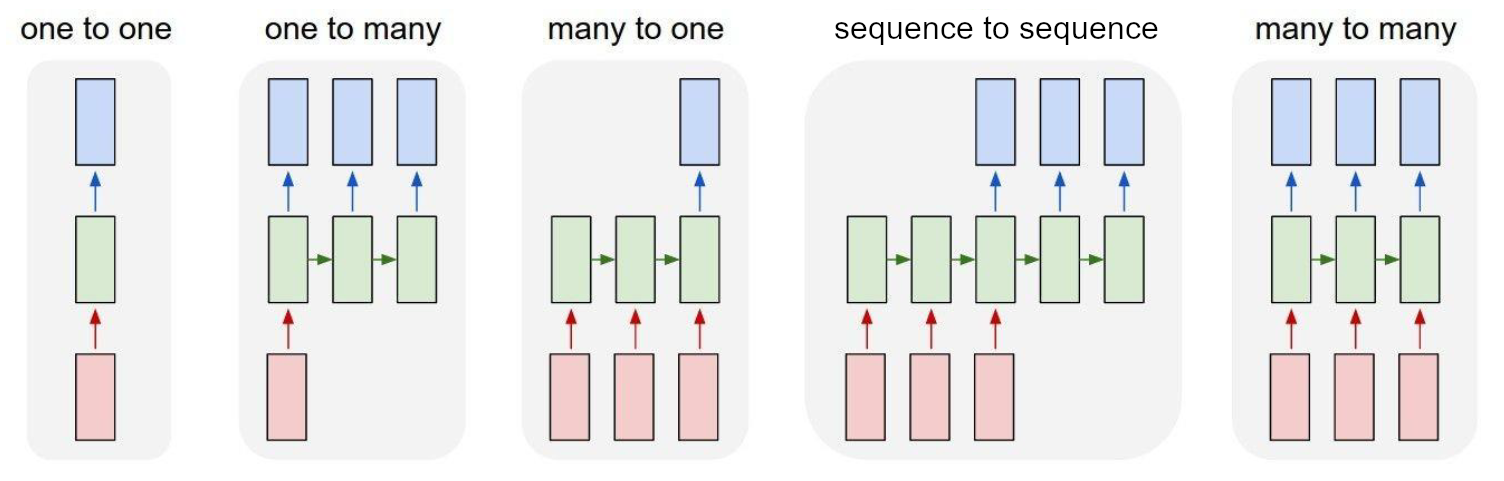
\includegraphics[width=0.7\linewidth]{images/many}
    \caption[Different kinds of NN]{Different kinds of Neural Networks}
    \label{fig:seq-many}
\end{figure}

It is also possible to apply sequential processing to non-sequence data for example to classify images by taking a series of ``glimpses'', or to generate images one piece at a time.

Moreover, sequences are particularly useful for forecasting. Trajectory forecasting is used in human robot interaction, long term tracking across occlusions, safety of autonomous vehicles. Other things to forecast with NNs are weather and natural disasters, market trends, critical pressure of a power plant, gas supply and demand.

There are many kinds of networks suitable for this task. We'll analyze them in the next sections.


\subsection{Convolutional Neural Networks for Sequences}\label{sec:seq-cnn}

CNNs present some problems when applied to sequences:
\begin{myitem}
    \item Fixed size and static input, but this issue can be resolved by concatenating more frames as input;
    \item The output is a single choice from a fixed list of options, however one may predict one word at a time or a fixed number of output words.
\end{myitem}

\textbf{Temporal Convolutional Networks} exploits CNNs' strengths to build a network with the following features:
\begin{myitem}
    \item Convolutions are causal;
    \item Dilation: 12 layers may process a history of size $2^{12}$;
    \item Easy to train and exceeding expectations;
    \item Needs compromise on flexibility (e.g. variable number of input frames);
    \item Trivial to parallelize (per layer);
    \item Exploits local dependencies;
    \item ``Interaction distance'' between positions linear or logarithmic.
\end{myitem}
The main issue with this approach is that long distance dependencies require many layers.


\subsection{Recurrent Neural Networks for Sequences}\label{sec:seq-rnn}

RNNs offer a lot of flexibility in all scenarios described above (see \ref{sec:sequence}).\\
The key idea is that RNNs have an \textit{internal state} that is updated as a sequence is processed. We can process a sequence of vectors $x$ by applying a recurrence formula at every time step:
\begin{equation}\label{eq:recurrence-rnn}
    \underbrace{h_t}_{\text{new state}} = \underbrace{f_W}_{\substack{\text{some function} \\ \text{with parameters } W}} (\underbrace{h_{t-1}}_{\text{old state}}, \underbrace{x_t}_{\substack{\text{input vector} \\ \text{at time step } t}})
\end{equation}
Notice that the same function and the same set of parameters (weight matrix) are used at every time step.


\subsubsection{RNN and LSTM models and their applications}\label{sec:seq-lstm}

The state of a simple RNN (also called \textit{Vanilla RNN} or \textit{Elman RNN}, see figure \ref{fig:seq-simple-rnn}) consists of a single hidden vector $h$:
\begin{flalign}\label{eq:rnn-hidden}
    h_t &= f_W (h_{t-1}, x_t)\\
        &\downarrow\\
    h_t &= \tanh(W_{hh} h_{t-1} + W_{xh} x_t)\\
    y_t &= W_{hy} h_t
\end{flalign}

\begin{figure}[h!]
    \centering
    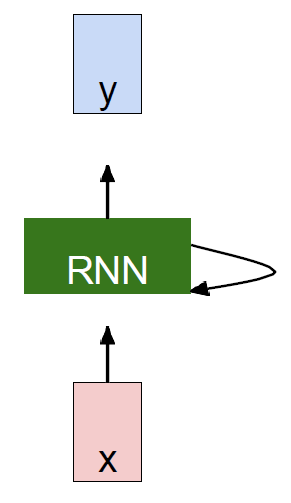
\includegraphics[width=0.15\linewidth]{images/seq-simple-rnn}
    \caption[Simple RNN]{Simple RNN}
    \label{fig:seq-simple-rnn}
\end{figure}

In figures \ref{fig:seq-many-many}, \ref{fig:seq-many-one}, \ref{fig:seq-one-many}, \ref{fig:seq-seq-seq} are shown the computational graphs for different kinds of RNNs. About the sequence-to-sequence RNN, it's worth to notice that it is the combination of a many-to-one RNN, which encodes the input sequence in a single output vector, and a one-to-many RNN, which produces an output sequence from the single input vector.

\begin{figure}[h!]
    \centering
    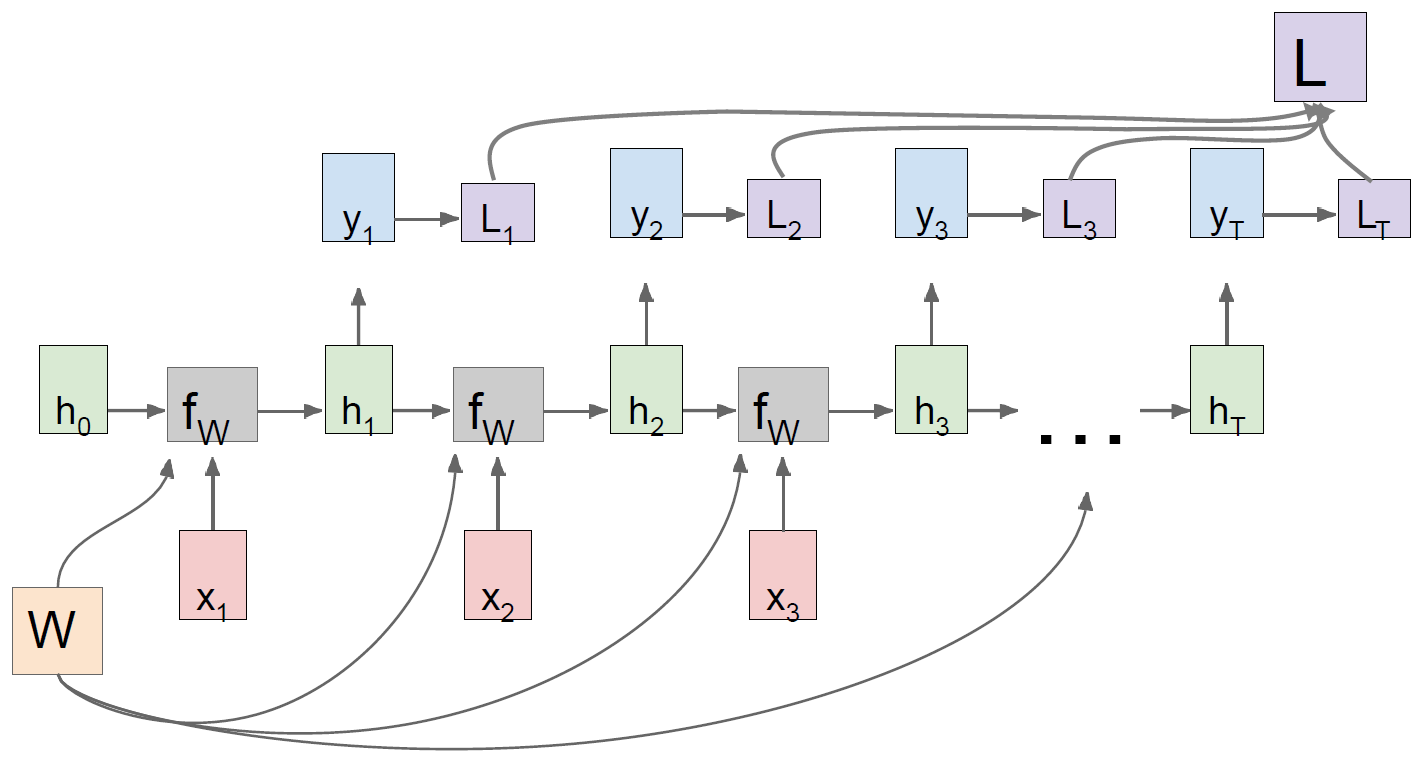
\includegraphics[width=0.6\linewidth]{images/seq-many-many}
    \caption[Many-to-many RNN]{Many-to-many RNN}
    \label{fig:seq-many-many}
\end{figure}

\begin{figure}[h!]
    \centering
    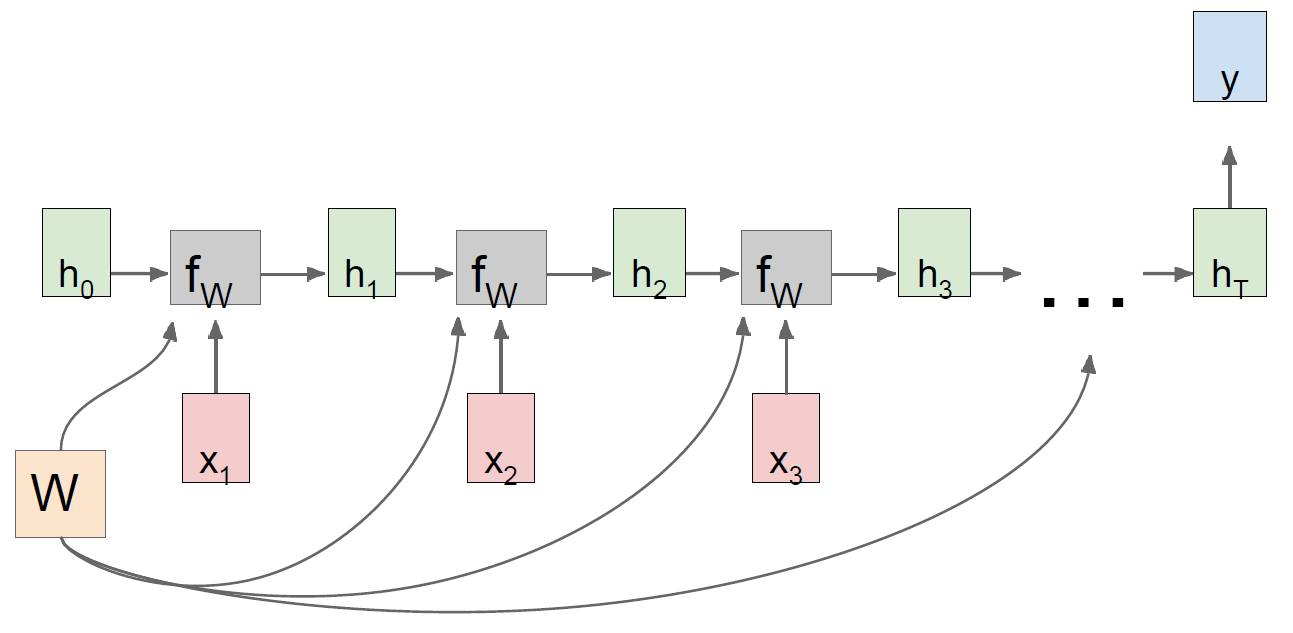
\includegraphics[width=0.6\linewidth]{images/seq-many-one}
    \caption[Many-to-one RNN]{Many-to-one RNN}
    \label{fig:seq-many-one}
\end{figure}

\begin{figure}[h!]
    \centering
    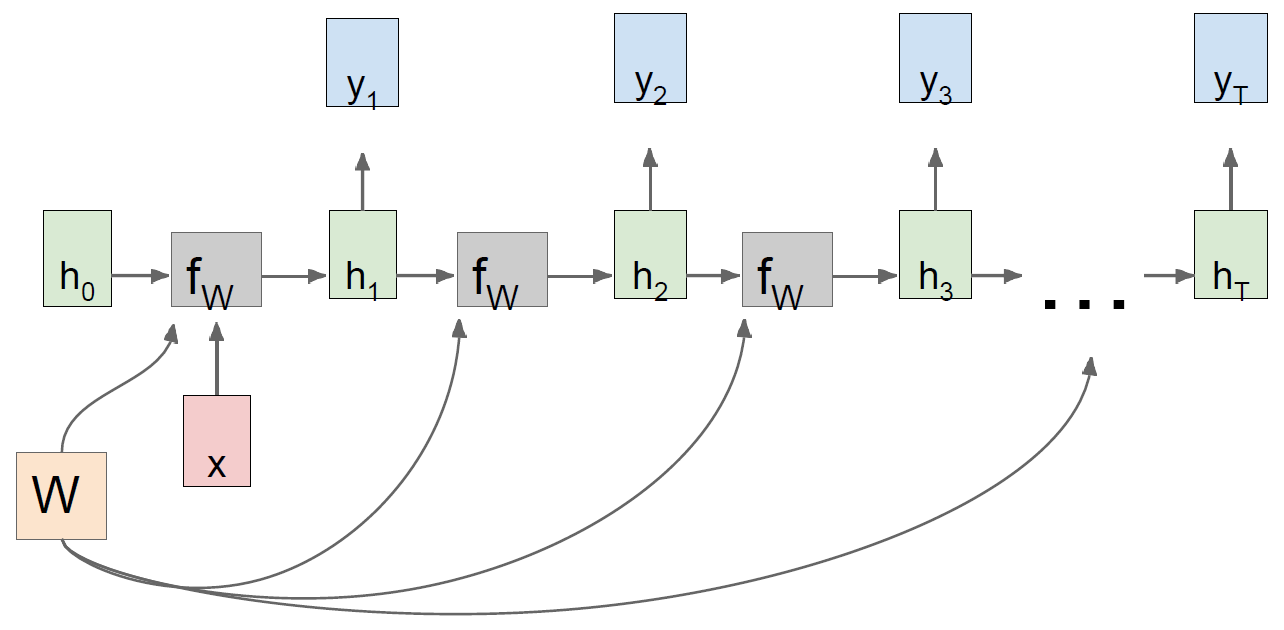
\includegraphics[width=0.6\linewidth]{images/seq-one-many}
    \caption[One-to-many RNN]{One-to-many RNN}
    \label{fig:seq-one-many}
\end{figure}

\begin{figure}[h!]
    \centering
    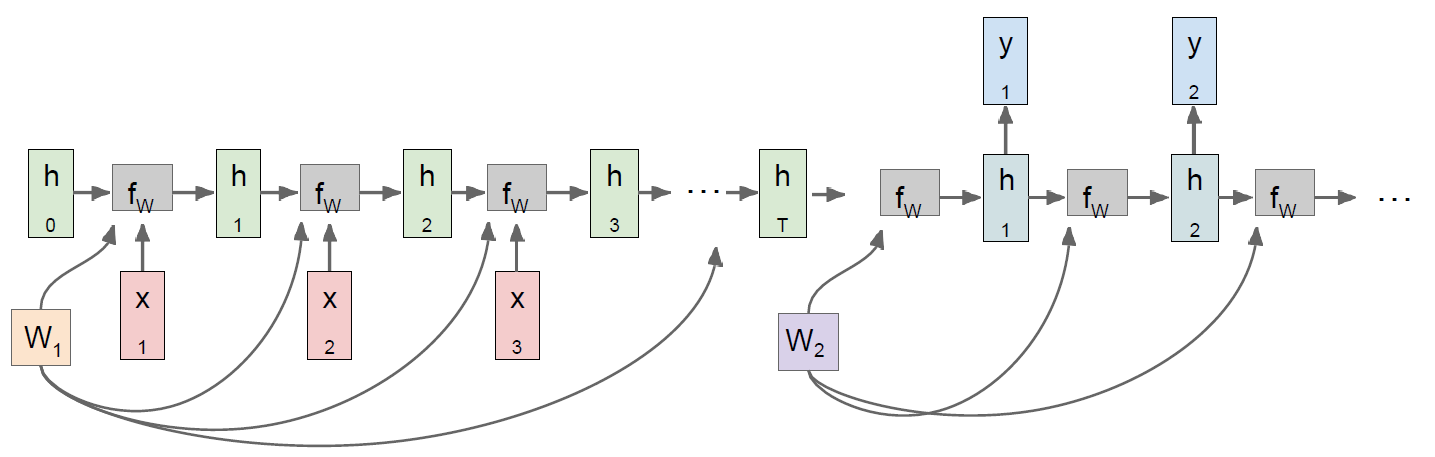
\includegraphics[width=0.6\linewidth]{images/seq-seq-seq-rnn}
    \caption[Sequence-to-sequence RNN]{Sequence-to-sequence RNN}
    \label{fig:seq-seq-seq}
\end{figure}

One interesting application of RNNs in NLP is to train \textbf{language models}, that is, to learn the probability for each work in the vocabulary to follow a given word (or set of words), based on a lot of sentences, for example from Wikipedia or from books:
\begin{equation}\label{eq:language-model}
    \Pr(\text{next word} | \text{previous words}).
\end{equation}

If we use a single word as \textit{history} to predict next word, we can have a RNN like the one in figure \ref{fig:seq-language}, where we give in input 300 learnable numbers associated with each words in the dataset, then we have a hidden layer $h_4 = \tanh(0, W_{hx} \cdot x_4 + W_{hh} \cdot h_3)$,  with 500-dimensional vectors, and finally the output vector $y_4 = W_{hy} \cdot h_4$ with 10,001-dimensional class scores produced by Softmax function over 10,000 words of the English vocabulary + 1 special \texttt{<END>} token.\\
We can use the trained language model to generate sentences, by sampling a word from each $y_i$ in the output vector, until the \texttt{<END>} token.

\begin{figure}[h!]
    \centering
    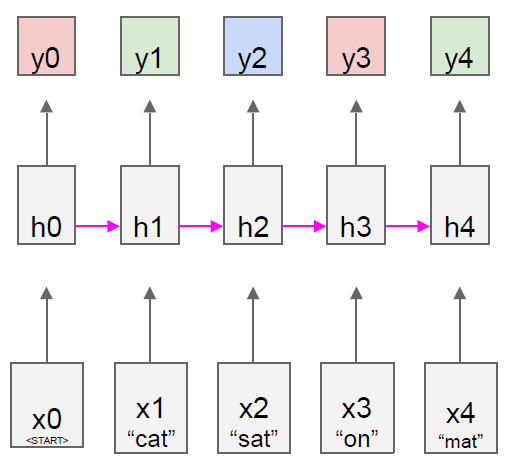
\includegraphics[width=0.3\linewidth]{images/seq-language}
    \caption[Example of RNN for training a language model.]{Example of RNN for training a language model.}
    \label{fig:seq-language}
\end{figure}

As shown in figures \ref{fig:seq-language1} and \ref{fig:seq-language2}, we can train and test a language model also at character level. At test time, it will be sufficient to sample characters one at a time, and feed them back to the model.

\begin{minipage}{.5\linewidth}
    \begin{figure}[H]
        \centering
        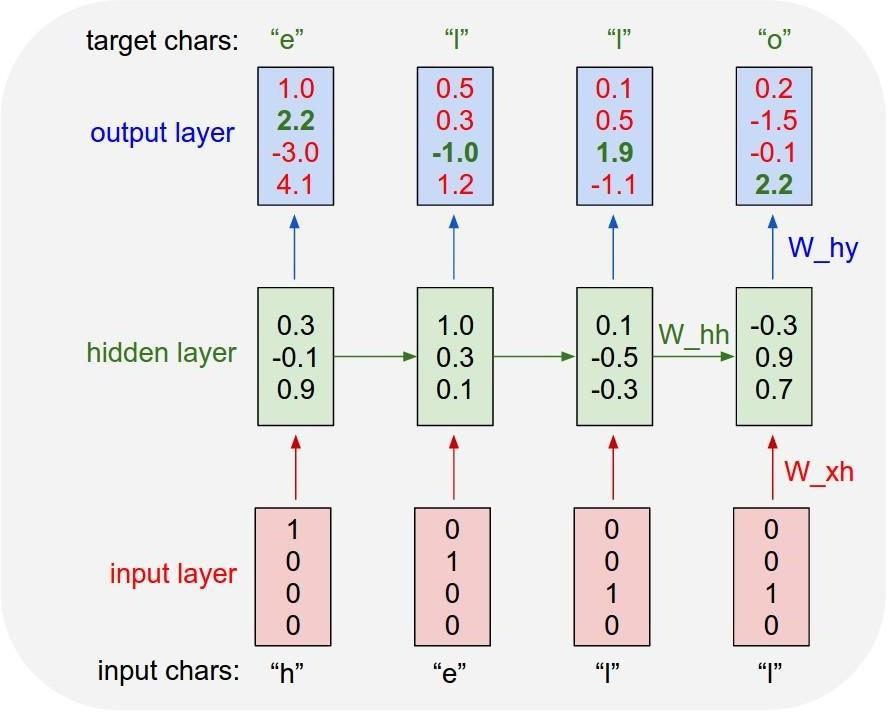
\includegraphics[width=0.8\linewidth]{images/seq-language1}
        \caption[Training a char-level language model]{Training a char-level language model}
        \label{fig:seq-language1}
    \end{figure}
\end{minipage}
\begin{minipage}{.5\linewidth}
    \begin{figure}[H]
        \centering
        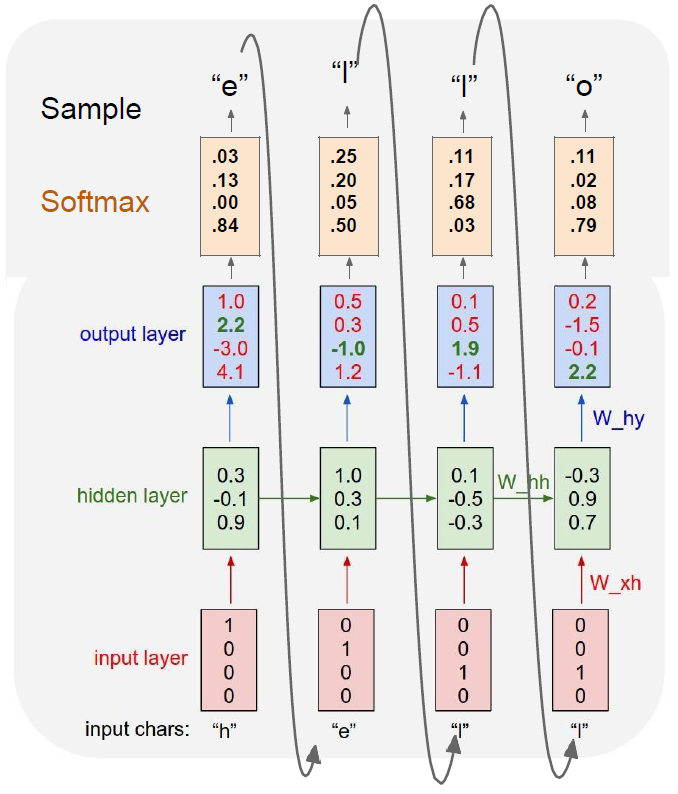
\includegraphics[width=0.7\linewidth]{images/seq-language2}
        \caption[Sampling from a char-level language model]{Sampling from a char-level language model}
        \label{fig:seq-language2}
    \end{figure}
\end{minipage}


In RNNs, we have two different possibility to perform backpropagation (see figures \ref{fig:seq-rnn-backpropagation} and \ref{fig:seq-rnn-backpropagation1}):
\begin{myenum}
    \item \textit{''Classic'' backpropagation}: Forward through entire sequence to compute loss, then backward through entire sequence to compute gradient;
    \item \textit{Truncated backpropagation}: Run forward and backward through chunks of the sequence instead of whole sequence. In this way, we carry hidden states forward in time for the whole training, but only backpropagate for some smaller number of steps.
\end{myenum}


\begin{minipage}{.5\linewidth}
    \begin{figure}[H]
        \centering
        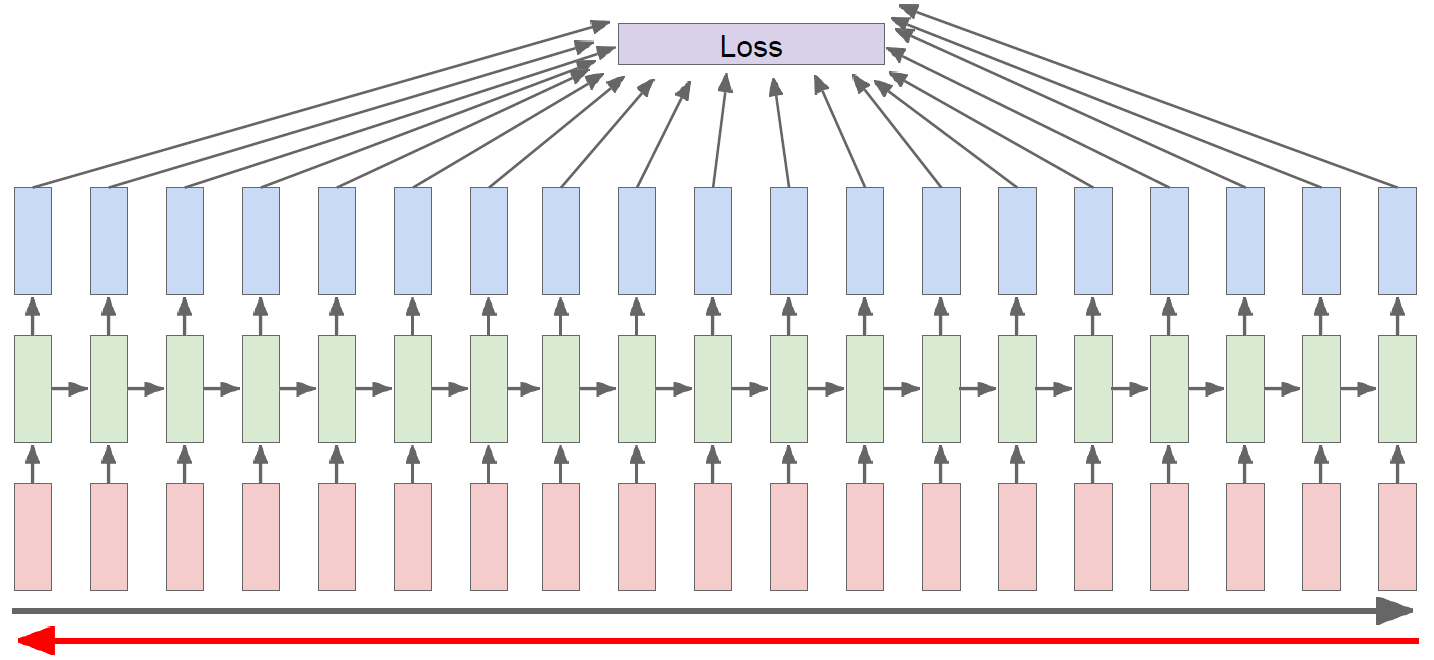
\includegraphics[width=0.8\linewidth]{images/seq-rnn-backpropagation}
        \caption[Classic Backpropagation in RNNs]{Classic Backpropagation in RNNs}
        \label{fig:seq-rnn-backpropagation}
    \end{figure}
\end{minipage}
\begin{minipage}{.5\linewidth}
    \begin{figure}[H]
        \centering
        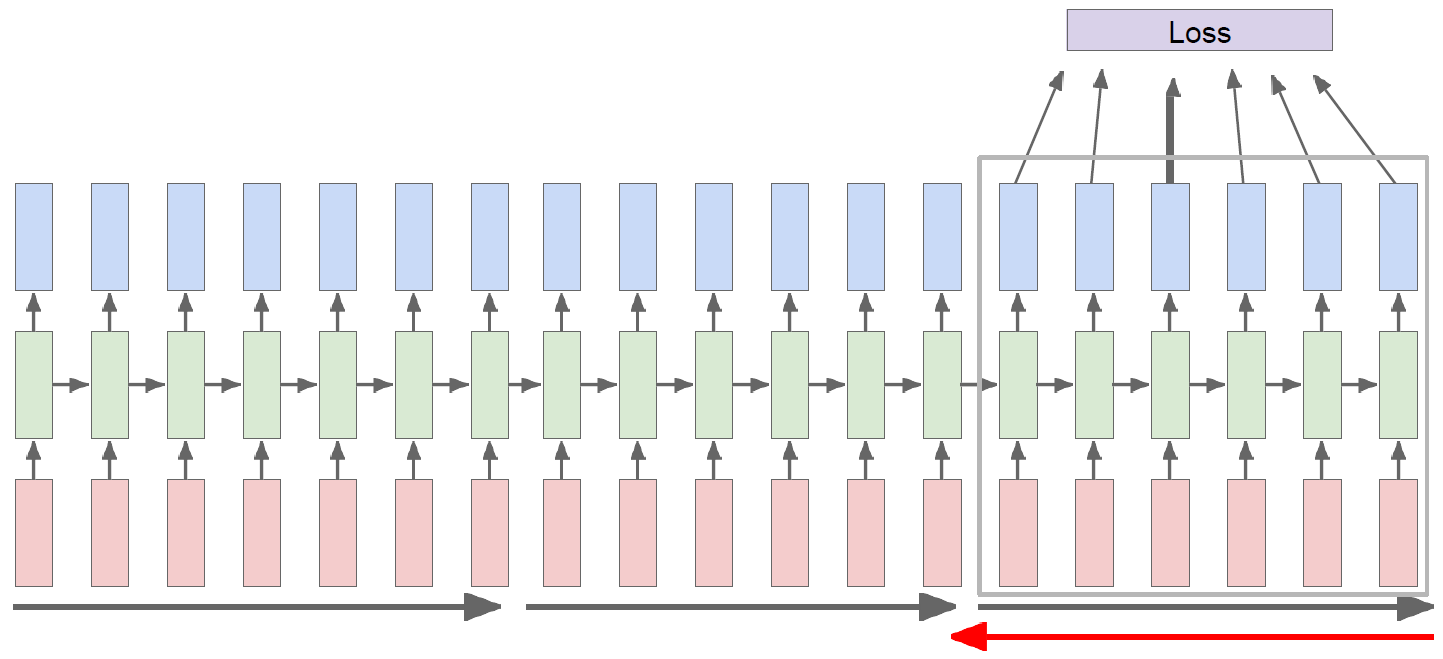
\includegraphics[width=0.8\linewidth]{images/seq-rnn-backpropagation1}
        \caption[Truncated Backpropagation in RNNs]{Truncated Backpropagation in RNNs}
        \label{fig:seq-rnn-backpropagation1}
    \end{figure}
\end{minipage}

Possible applications of sentence generation are: generation of sonnets or code, image captioning, visual question answering. In some cases, it is possible to give an interpretation to cells to find, for example, quote detection cells, line length tracking cells, if statement cells, comment cells, code depth cells...
\newpage
For \textbf{image captioning}, the input image is passed through a CNN, whose output layer (fully connected + softmax) is removed, and the result is given in input to a RNN, with hidden layer $h = \tanh(W_{xh} \cdot x + W_{hh} \cdot h + W_{ih} \cdot v)$, where $W_{ih} \cdot v$ comes from the CNN's output. For this task, as well as for \textbf{visual question answering}, better results can be obtained using \textbf{Attention mechanisms}. By weighting the features, the RNN focuses its attention at different spatial location when generating each word, or when answering to each question (see figures \ref{fig:seq-attention1} and \ref{fig:seq-attention2}).

\begin{minipage}{.6\linewidth}
    \begin{figure}[H]
        \centering
        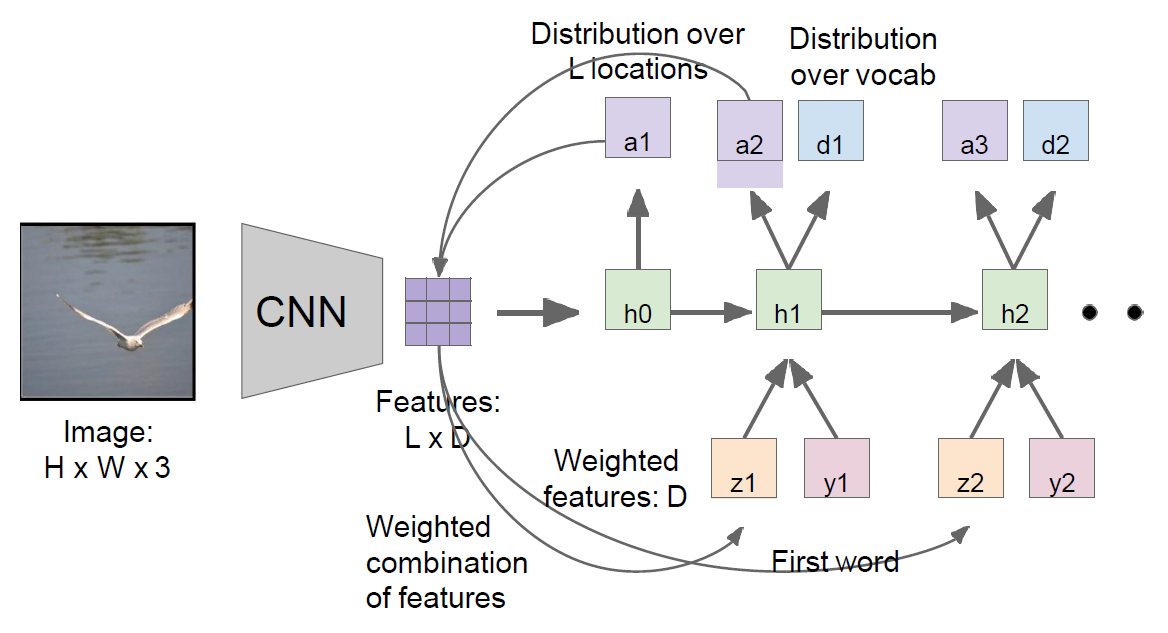
\includegraphics[width=0.9\linewidth]{images/seq-attention1}
        \caption[Image Captioning with Attention]{Image Captioning with Attention}
        \label{fig:seq-attention1}
    \end{figure}
\end{minipage}
\begin{minipage}{.4\linewidth}
    \begin{figure}[H]
        \centering
        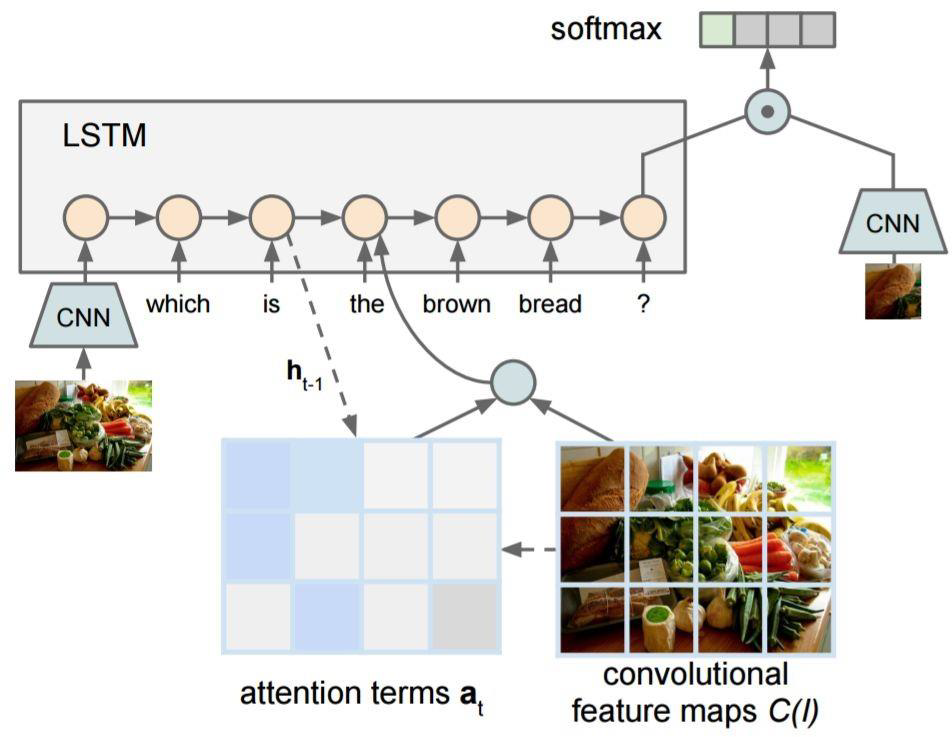
\includegraphics[width=0.8\linewidth]{images/seq-attention2}
        \caption[Question Answering with Attention]{Question Answering with Attention}
        \label{fig:seq-attention2}
    \end{figure}
\end{minipage}

As we saw in equation \ref{eq:rnn-hidden}, in a vanilla multilayer RNN, we have
\begin{flalign}\label{eq:rnn-hidden1}
    h_t &= \tanh(W_{hh}h_{t-1} + W_{xh}x_t)\\
        &= \tanh\left((W_{hh}W_{hx})\binom{h_{t-1}
        }{x_t}\right)\\
        &= \tanh\left(W\binom{h_{t-1}}{x_t}\right)
\end{flalign}
So, the backpropagation from $h_t$ to $h_{t-1}$ multiplies by $W$. Thus, computing gradient of $h_0$ involves many factors of $W$ and repeated $\tanh$ (see figure \ref{fig:seq-rnn-gradients}). This can lead to \textit{exploding gradients} if the largest singular value is $>1$, or to \textit{vanishing gradients} if it is $<1$. The first issue can be solved with \textbf{gradient clipping}, i.e., scaling gradient if its norm is too big; the second one require to change RNN architecture, and that's why LSTMs exist.

\begin{figure}[h!]
    \centering
    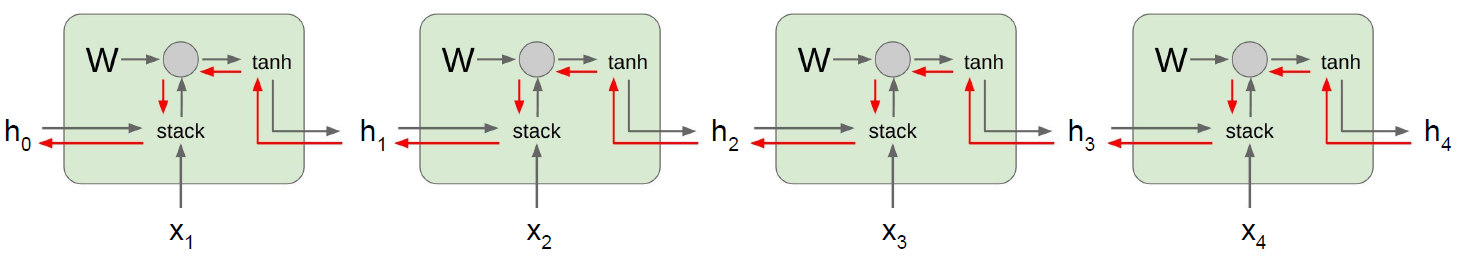
\includegraphics[width=0.7\linewidth]{images/seq-rnn-gradients}
    \caption[Backpropagation in vanilla RNNs]{Backpropagation in vanilla RNNs}
    \label{fig:seq-rnn-gradients}
\end{figure}

In \textbf{Long Short Term Memory} networks, the hidden layer becomes
\begin{flalign}\label{eq:lstm-hidden}
    \begin{pmatrix}
        i\\f\\o\\g
    \end{pmatrix} &=
    \begin{pmatrix}
        \sigma\\ \sigma\\ \sigma\\ \tanh
    \end{pmatrix}
    W \binom{h_{t-1}}{x_t}\\
    c_t &= f \cdot c_{t-1} + i \cdot g\\
    h_t &= o \cdot \tanh(c_t)
\end{flalign}
where $i$ is the \textit{input gate}, that decides whether to write to a cell, $f$ is the \textit{forget gate}, that decides whether to erase a cell, $o$ is the \textit{output gate}, that decided how much to reveal a cell, and $g$ is the \textit{gate gate}, that decides how much to write to a cell. Thus, the backpropagation from $c_t$ to $c_{t-1}$ is only an elementwise multiplication by $f$, without any matrix multiplication by $W$, so we can have an uninterrupted gradient flow from $c_n$ to $c_0$, as shown in figure \ref{fig:seq-lstm-gradients}. Notice that this behavior is somehow similar to \textit{ResNet}'s.
\begin{figure}[h!]
    \centering
    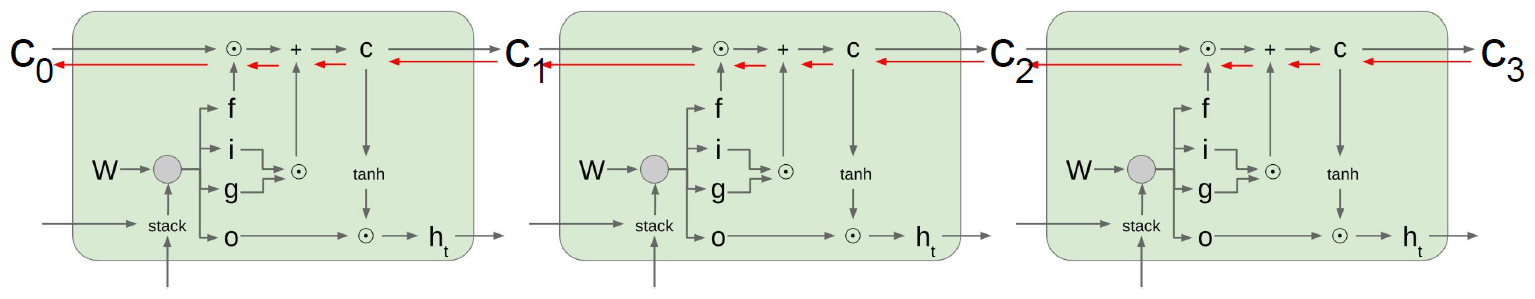
\includegraphics[width=0.7\linewidth]{images/seq-lstm-gradients}
    \caption[Backpropagation in LSTMs]{Backpropagation in LSTMs}
    \label{fig:seq-lstm-gradients}
\end{figure}

Other RNN variants are \textbf{GRU} and \textbf{MUT1/2/3}. Let's see GRU's structure:
\begin{flalign}\label{eq:gru-hidden}
    r_t &= \sigma(W_{xr}x_t + W_{hr}h_{t-1} + b_r)\\
    z_t &= \sigma(W_{xz}x_t + W_{hz}h_{t-1} + b_z)\\
    \tilde{h}_t &= \tanh(W_{xh}x_t + W_{hh}(r_t \cdot h_{t-1}) + b_r)\\
    h_t &= z_t \cdot h_{t-1} + (1-z_t) \cdot \tilde{h}_t
\end{flalign}

To conclude about RNN models, we have to say that better/simpler architectures are a hot topic of current research, as well as new paradigms for reasoning over sequences.


\subsubsection{Modelling multiple agents and the scene}\label{sec:seq-multiple-agents}

Now we'll spend some more words about \textbf{Trajectory Forecasting}, or \textit{predicting unpredictable people}. The goal is to predict future positions, given previous positions.

We'll analyze this topic through its three key aspects:
\begin{myitem}
    \item \textbf{Social interaction} (groups and collision avoidance): combine results from an LSTM for each person by using \textit{social pooling} to exploit the knowledge that each individual is influenced by the surrounding people (see figure \ref{fig:seq-trajectory-1});
    \item \textbf{People's attention} (head pose):
    \begin{itemize}
        \item \textit{MX-LSTM} use people oriented velocity and head pose jointly to forecast people motion,
        \item Based on sociological findings and data statistics,
        \item The input of the LSTM is a combination of input position and head pose, optimized via log Choleski factorization,
        \item Head pose can be applied to social pooling too;
    \end{itemize}
    \item \textbf{The context} (scene): the scene, usually encoded by a CNN, constraints the plausible motion.
\end{myitem}

\begin{figure}[H]
    \centering
    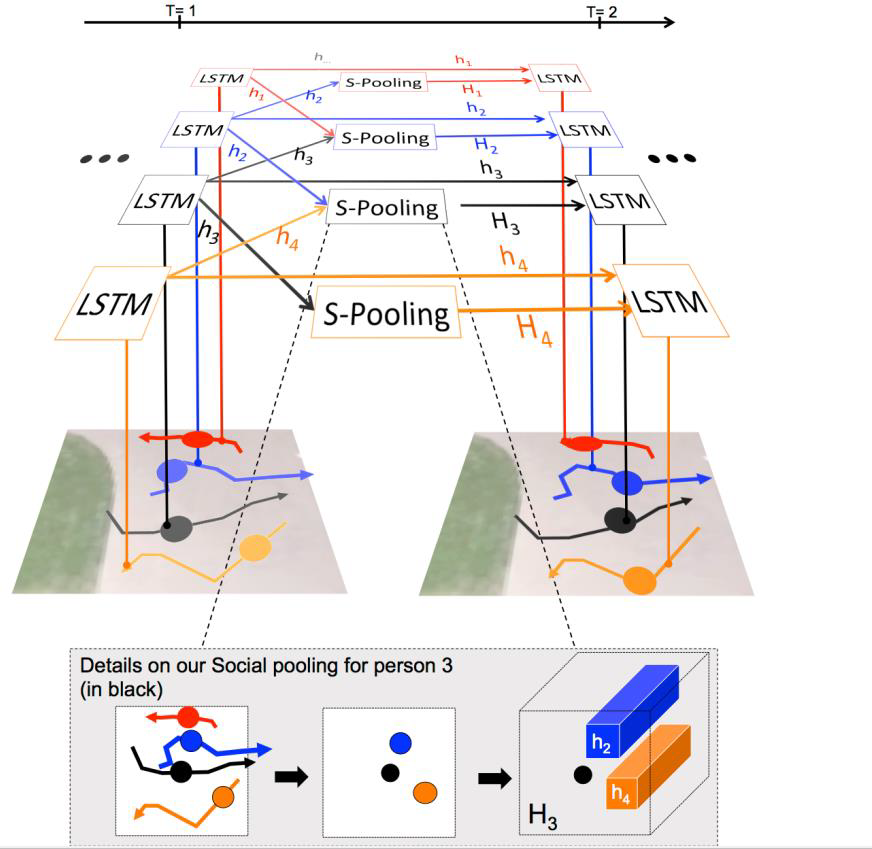
\includegraphics[width=.4\linewidth]{images/seq-trajectory-1}
    \caption[Social pooling in trajectory forecasting]{Social pooling in trajectory forecasting}
    \label{fig:seq-trajectory-1}
\end{figure}


\subsection{Transformer Networks for Sequences}\label{sec:seq-transformers}

As we saw in previous sections, to learn representations of variable length data, essential for sequence-to-sequence learning, we can use LSTMs or GRUs, but they present some issues:
\begin{myitem}
    \item They use \textit{sequential computation} to transfer knowledge from the first elements of a sequence to the next, but this approach inhibits parallelization;
    \item They don't have any explicit modeling of long and short range dependencies;
    \item We want model hierarchy.
\end{myitem}

On the other hand, CNNs have many advantages (such as easy per layer parallelizability, exploitation of local dependencies, \textit{interaction distance} between positions linear or logarithmic), but their long-distance dependencies require many layers.

Since we know that attention between encoder and decoder is crucial in \textit{Neural Machine Translation}, we can apply the same idea for representations: \textbf{Self-Attention} introduces interesting improvements over RNNs and CNNs (see also figure \ref{fig:seq-self-attention}):
\begin{myitem}
    \item Constant path length between any two positions;
    \item Gating/multiplicative interactions;
    \item Trivial to parallelize (per layer).
\end{myitem}

\begin{figure}[h!]
    \centering
    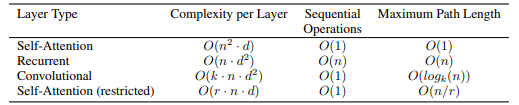
\includegraphics[width=0.7\linewidth]{images/seq-self-attention}
    \caption[Self Attention VS RNNs VS CNNs]{Self Attention VS RNNs VS CNNs}
    \label{fig:seq-self-attention}
\end{figure}

The \textbf{Transformer} is a very successful encoder-decoder network that use this approach. In figures \ref{fig:seq-transformer-1} and \ref{fig:seq-transformer-2} is shown its architecture at higher and lower level: the last encoder sends the representations of the input words it computed to all the decoders, thus giving them a \textit{memory}.

\begin{minipage}{.4\linewidth}
    \begin{figure}[H]
        \centering
        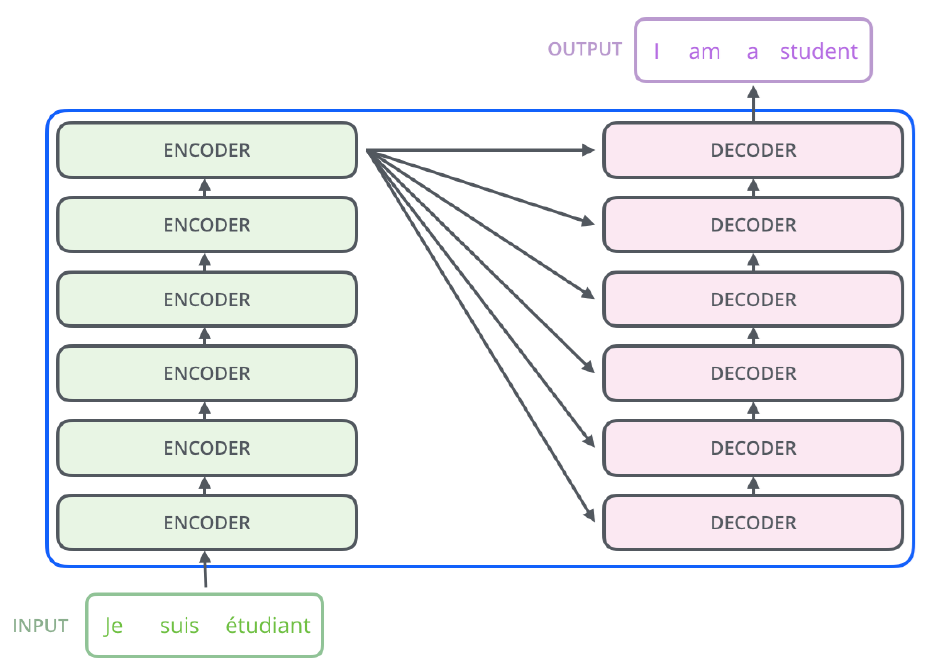
\includegraphics[width=0.95\linewidth]{images/seq-transformer-1}
        \caption[Trasnsformer architecture (a)]{Trasnsformer architecture (a)}
        \label{fig:seq-transformer-1}
    \end{figure}
\end{minipage}
\begin{minipage}{.6\linewidth}
    \begin{figure}[H]
        \centering
        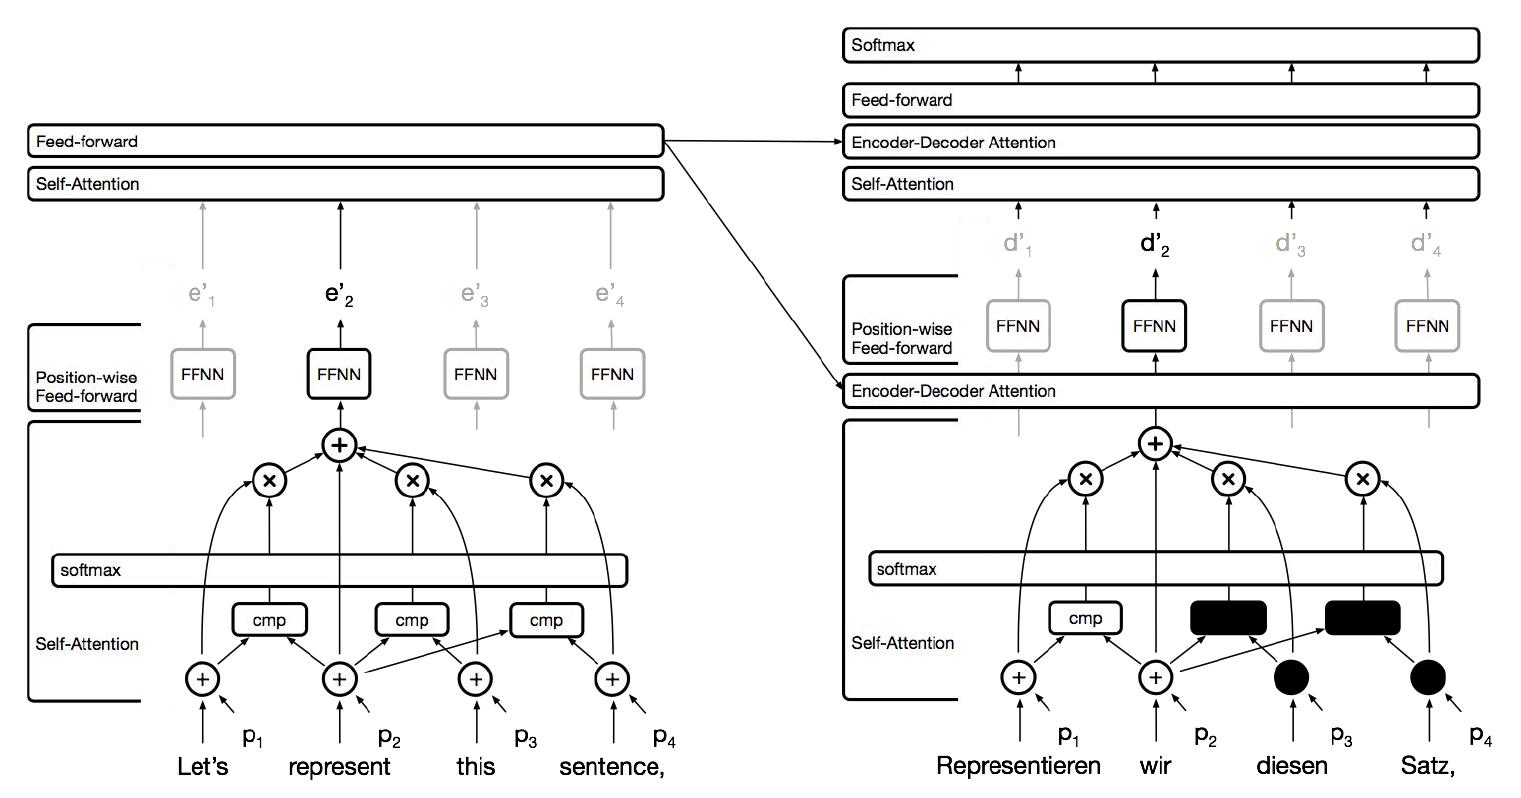
\includegraphics[width=0.95\linewidth]{images/seq-transformer-2}
        \caption[Transformer architecture (b)]{Transformer architecture (b)}
        \label{fig:seq-transformer-2}
    \end{figure}
\end{minipage}

Attention value is a function of $Q$ (the query), $K$ (the key) and $V$ (the value):
\begin{equation}\label{eq:attention}
A(Q,K,V) = softmax\left(\frac{QK^T}{\sqrt{d_k}}\right) V
\end{equation}
That is, $A$ uses softmax to give a weighted average of probabilities, where weights are given by the inputs, so that the output of a certain word depends mostly on words to which it is more tightly related, rather than closer ones. So, this approach is also invariant to word order. With \textit{multi-head attention}, parallel attention layers with different linear transformations on input and output are applied to each word.\\
It is important to notice that the self-attention blocks are different in encoders and decoders, as shown in figures \ref{fig:seq-transformer-5} and \ref{fig:seq-transformer-6}: in the encoders, the output originated from a word, depend on previous and next words, while in decoders, next words are masked, so that only previous words are considered; furthermore, in decoders, keys and values come from the last encoder, while queries from the previous decoder.

\begin{minipage}{.5\linewidth}
    \begin{figure}[H]
        \centering
        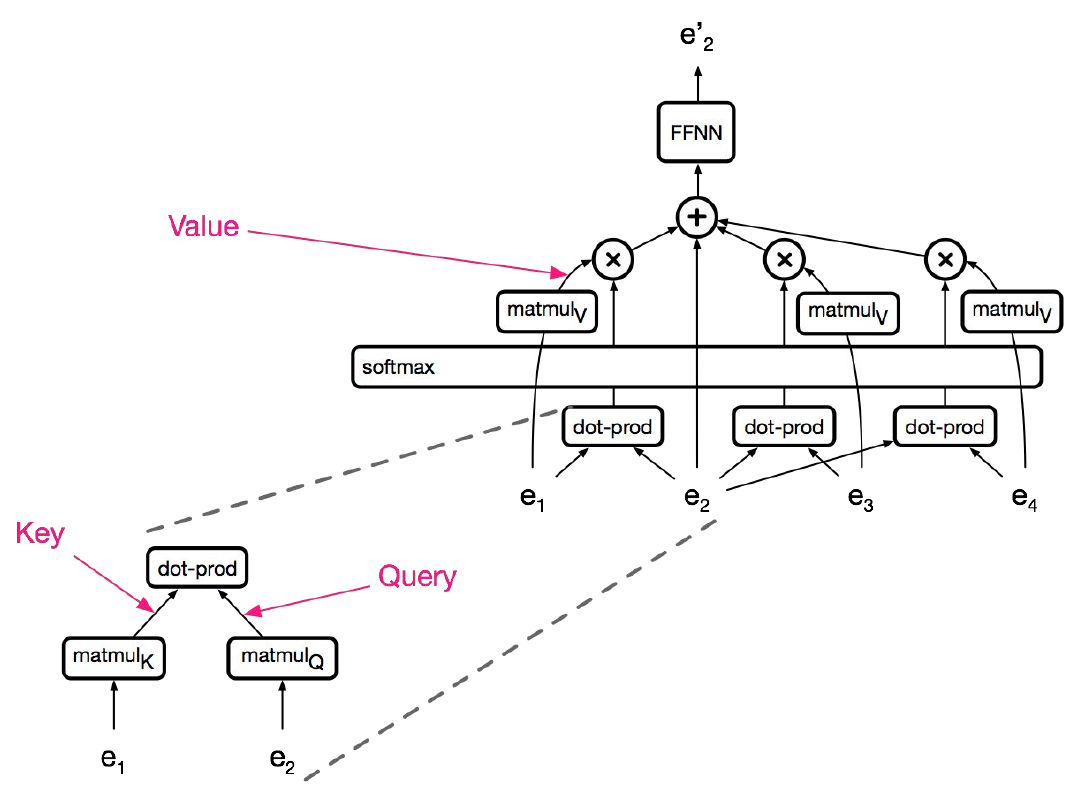
\includegraphics[width=0.95\linewidth]{images/seq-transformer-5}
        \caption[Encoder Self-Attention]{Encoder Self-Attention}
        \label{fig:seq-transformer-5}
    \end{figure}
\end{minipage}
\begin{minipage}{.5\linewidth}
    \begin{figure}[H]
        \centering
        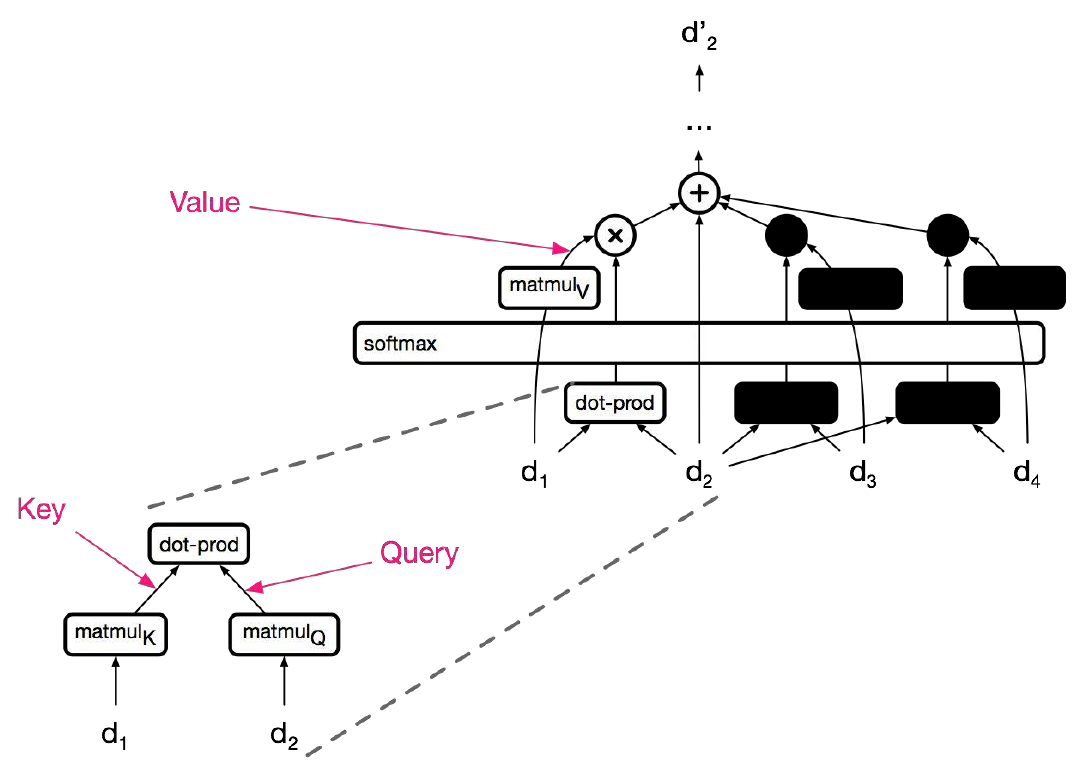
\includegraphics[width=0.95\linewidth]{images/seq-transformer-6}
        \caption[Decoder Self Attention]{Decoder Self Attention}
        \label{fig:seq-transformer-6}
    \end{figure}
\end{minipage}

The Transformer works in steps, described in figures \ref{fig:seq-transformer-3} and \ref{fig:seq-transformer-4}:
\begin{myitem}
    \item \textit{Step 1}: compute $K$ and $V$ from the input;
    \item \textit{Step 2}: combine $Q$ from the output with $K$ and $V$, autoregressively.
\end{myitem}

\begin{minipage}{.5\linewidth}
\begin{figure}[H]
    \centering
    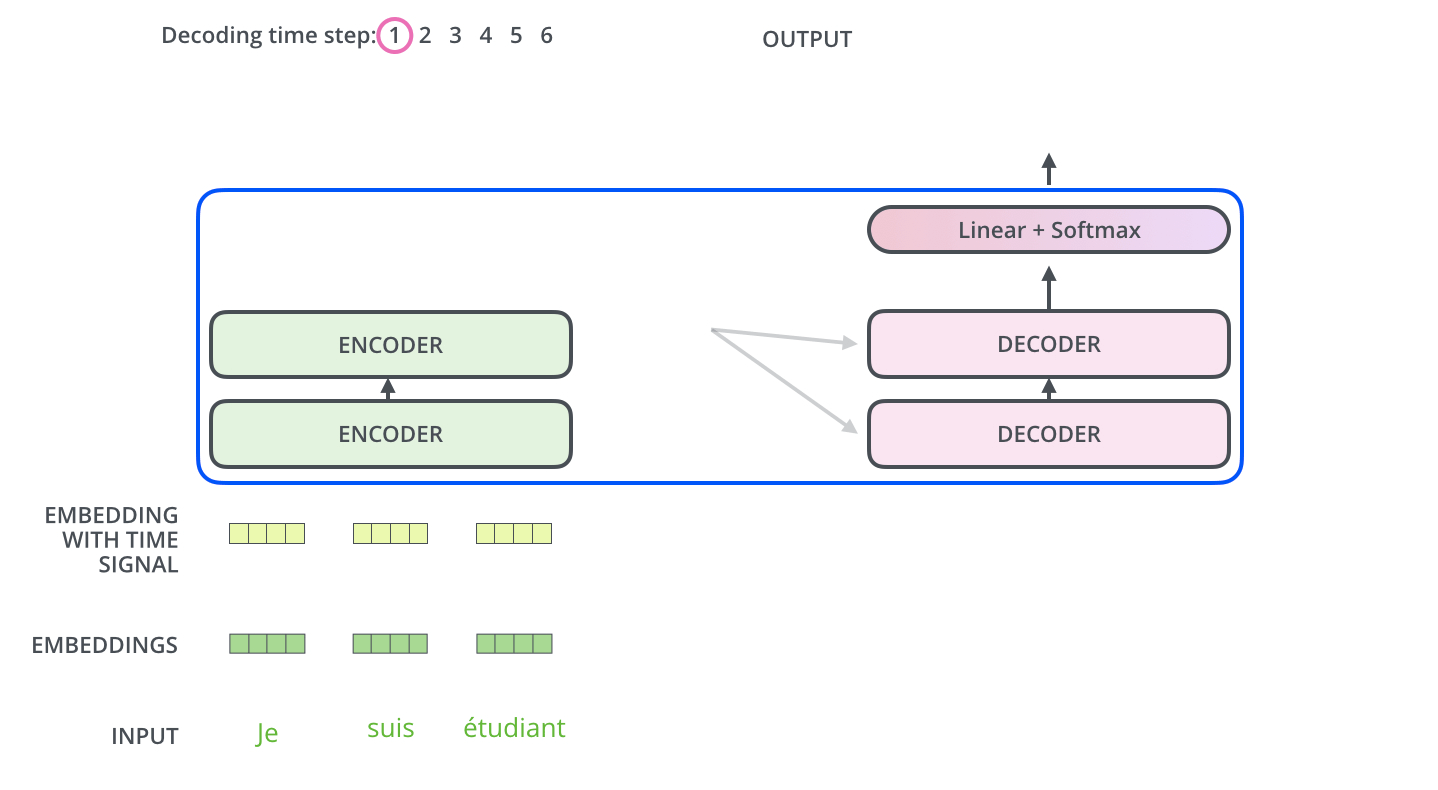
\includegraphics[width=0.95\linewidth]{images/seq-transformer-3}
    \caption[Transformer - step 1]{Transformer - step 1}
    \label{fig:seq-transformer-3}
\end{figure}
\end{minipage}
\begin{minipage}{.5\linewidth}
    \begin{figure}[H]
        \centering
        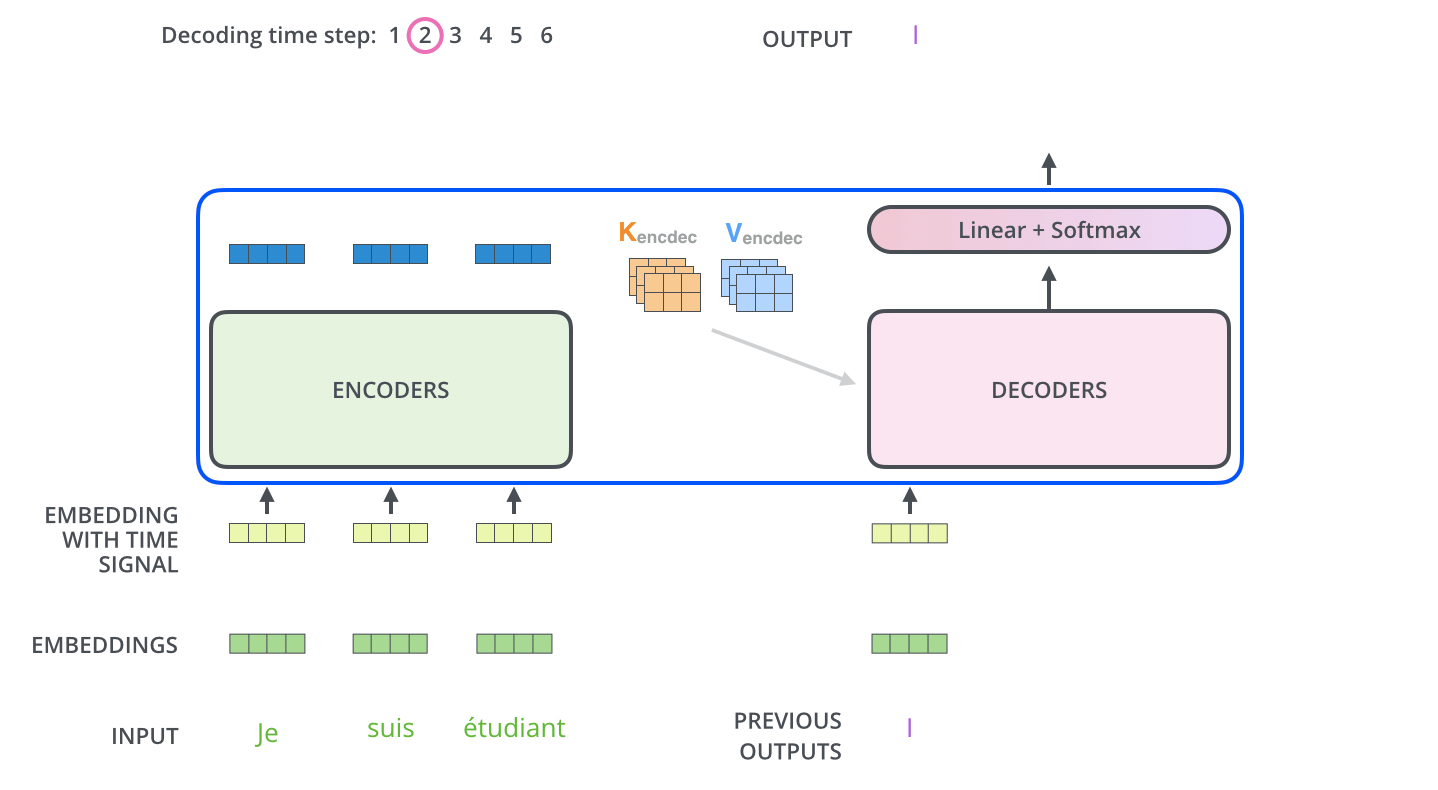
\includegraphics[width=0.95\linewidth]{images/seq-transformer-4}
        \caption[Trasnformer - step 2]{Trasnformer - step 2}
        \label{fig:seq-transformer-4}
    \end{figure}
\end{minipage}

As we said before, self-attention mechanism is permutation invariant to word order. But, if the ordering is relevant, the relative position of each word can be encoded in the input (see figure \ref{fig:seq-transformer-7}). It's important to note that Residuals (a structure similar to the one used in ResNet, shown in figure \ref{fig:seq-transformer-8}) are fundamental for position representation, since they carry positional information to higher layers, among other information.

\begin{minipage}{.6\linewidth}
    \begin{figure}[H]
        \centering
        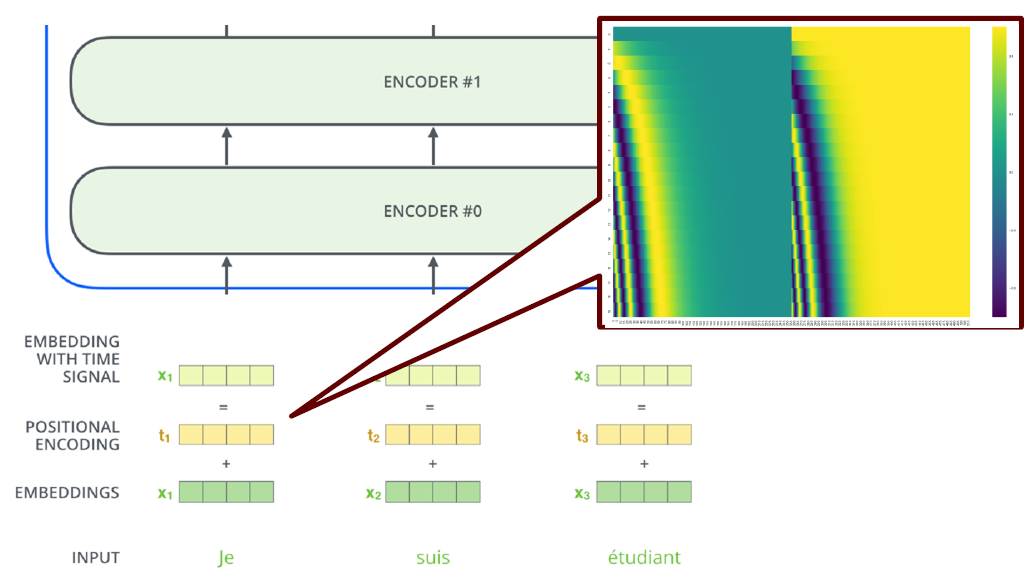
\includegraphics[width=0.95\linewidth]{images/seq-transformer-7}
        \caption[Transformer with positional encoding]{Transformer with positional encoding}
        \label{fig:seq-transformer-7}
    \end{figure}    
\end{minipage}
\begin{minipage}{.4\linewidth}
    \begin{figure}[H]
        \centering
        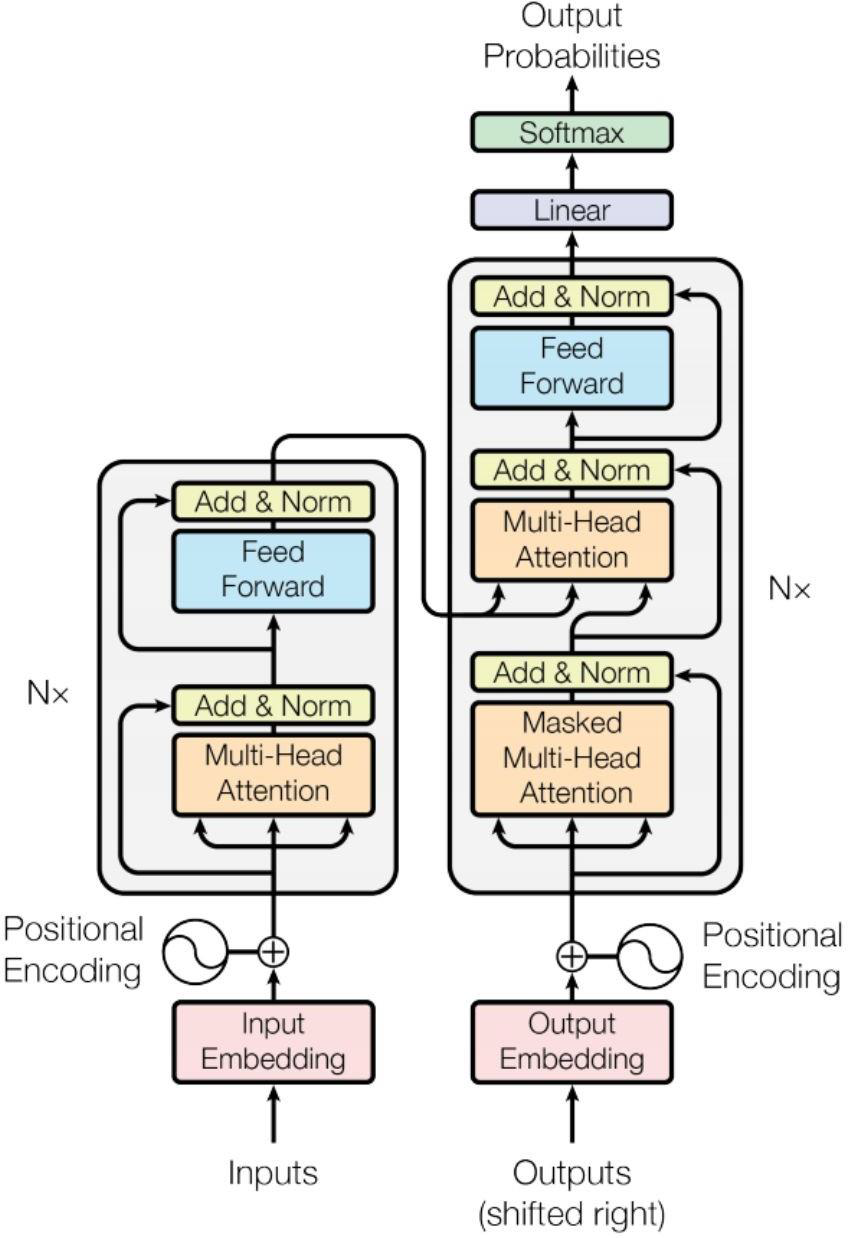
\includegraphics[width=0.7\linewidth]{images/seq-transformer-8}
        \caption[Transformer architecture (c)]{Transformer architecture (c)}
        \label{fig:seq-transformer-8}
    \end{figure}
\end{minipage}

Training details for Transformers:
\begin{myitem}
    \item ADAM optimizer with a learning rate warmup (warmup + exponential decay);
    \item Dropout during training at every layer just before adding residual;
    \item Layer norm;
    \item Attention dropout;
    \item Checkpoint averaging;
    \item Label smoothing;
    \item Auto-regressive decoding with beam search and length biasing.
\end{myitem}


\subsubsection{Self-Similarity, Image and Music Generation}\label{sec:seq-self-similarity}

Self-similarity is a property of images and music, for which portions (\textit{motifs}) repeat immediately or at a distance. This property can be exploited for \textbf{non-local means}: the attention window is restricted to local neighborhoods (good assumption thanks to spatial locality), but more relevance is given to most similar pixels, via a weighted average. This leads to the creation of \textbf{Image Transformers}, where positional encoding is based on pixel coordinates. \textbf{Relative attention} provides expressive timing, equivariance, and extends naturally to graphs, by combining multi-head attention and convolution:
\begin{equation}\label{eq:relative-attention}
    RA = softmax(QK^T + Qf(E_{rel}))
\end{equation}

Examples of application of these principles are:
\begin{myitem}
    \item \textit{Probabilistic image generation}:
    \begin{itemize}
        \item Model the joint distribution of pixels;
        \item Turn it into a sequence modeling problem
        \item Assigning probabilities allows measuring generalization;
        \item CNNs with gating match RNNs in quality, but are much faster due to parallelization;
        \item Modeling long range dependencies (important for big images) with CNNs requires either many layers (harder training) or large kernels (large parameter/computational cost).
    \end{itemize}
    \item \textit{Texture synthesis}: analyze similarities to reproduce a pattern;
    \item \textit{Denoising}: exploit similarities among close pixels to remove noise from an image;
    \item \textit{Super-Resolution}: enhance the resolution of an image;
    \item \textit{Unconditional and Conditional Image generation};
    \item \textit{Text to speech};
    \item \textit{Pentagram to music};
    \item \textit{Music models} to continue a given initial motif.
\end{myitem}


\subsubsection{Pre-trained Language Models}\label{sec:seq-pre-trained}

Language models only use left context or right context, for two reasons:
\begin{myenum}
    \item Directionality is needed to generate a well formed probability distribution;
    \item Words could “see themselves” in a bidirectional encoder.
\end{myenum}
But language understanding is bidirectional. To solve this problem, we can use \textbf{Masked Language Models}: mask out $k\%$ of the input words, and then predict the masked words. As usual, we need to find a trade-off for the size of $k$: if it is too little, the model is too expensive to train, if it is too big, we don't have enough context.\\
This approach introduces a problem: the \texttt{mask} token is never seen at fine-tuning time. A possible solution is to select $k\%$ of the words to predict, but don't replace always with \texttt{mask} token, instead:
\begin{myitem}
    \item 80\% of the time, replace with \texttt{mask} token,
    \item 10\% of the time, replace with a random word,
    \item 10\% of the time, keep same.
\end{myitem}

\textbf{Next Sentence Prediction}: to learn relationships between sentences, predict whether Sentence $B$ is actual sentence that proceeds Sentence $A$, or a random sentence. The input is represented by tokens that are sum of three embeddings: token embedding (which represents the word in the sentence), segment embedding (which says if a word belongs to $A$ or $B$) and position embedding (which describe the position of the word in the sentences). Single sequence is much more efficient.

\textbf{BERT} is a \textit{Bidirectional transformer} that can be pretrained on couples of sentences, and fine-tuned to perform different tasks, such as question answering, sentence classification or sentence tagging (see figure \ref{fig:seq-bert}). SQuAD is the model for question-answering fine-tuning, it uses token 0 (\texttt{CLS}) to emit logit for ``no answer'', which directly compete with answer span.

\begin{figure}[h!]
    \centering
    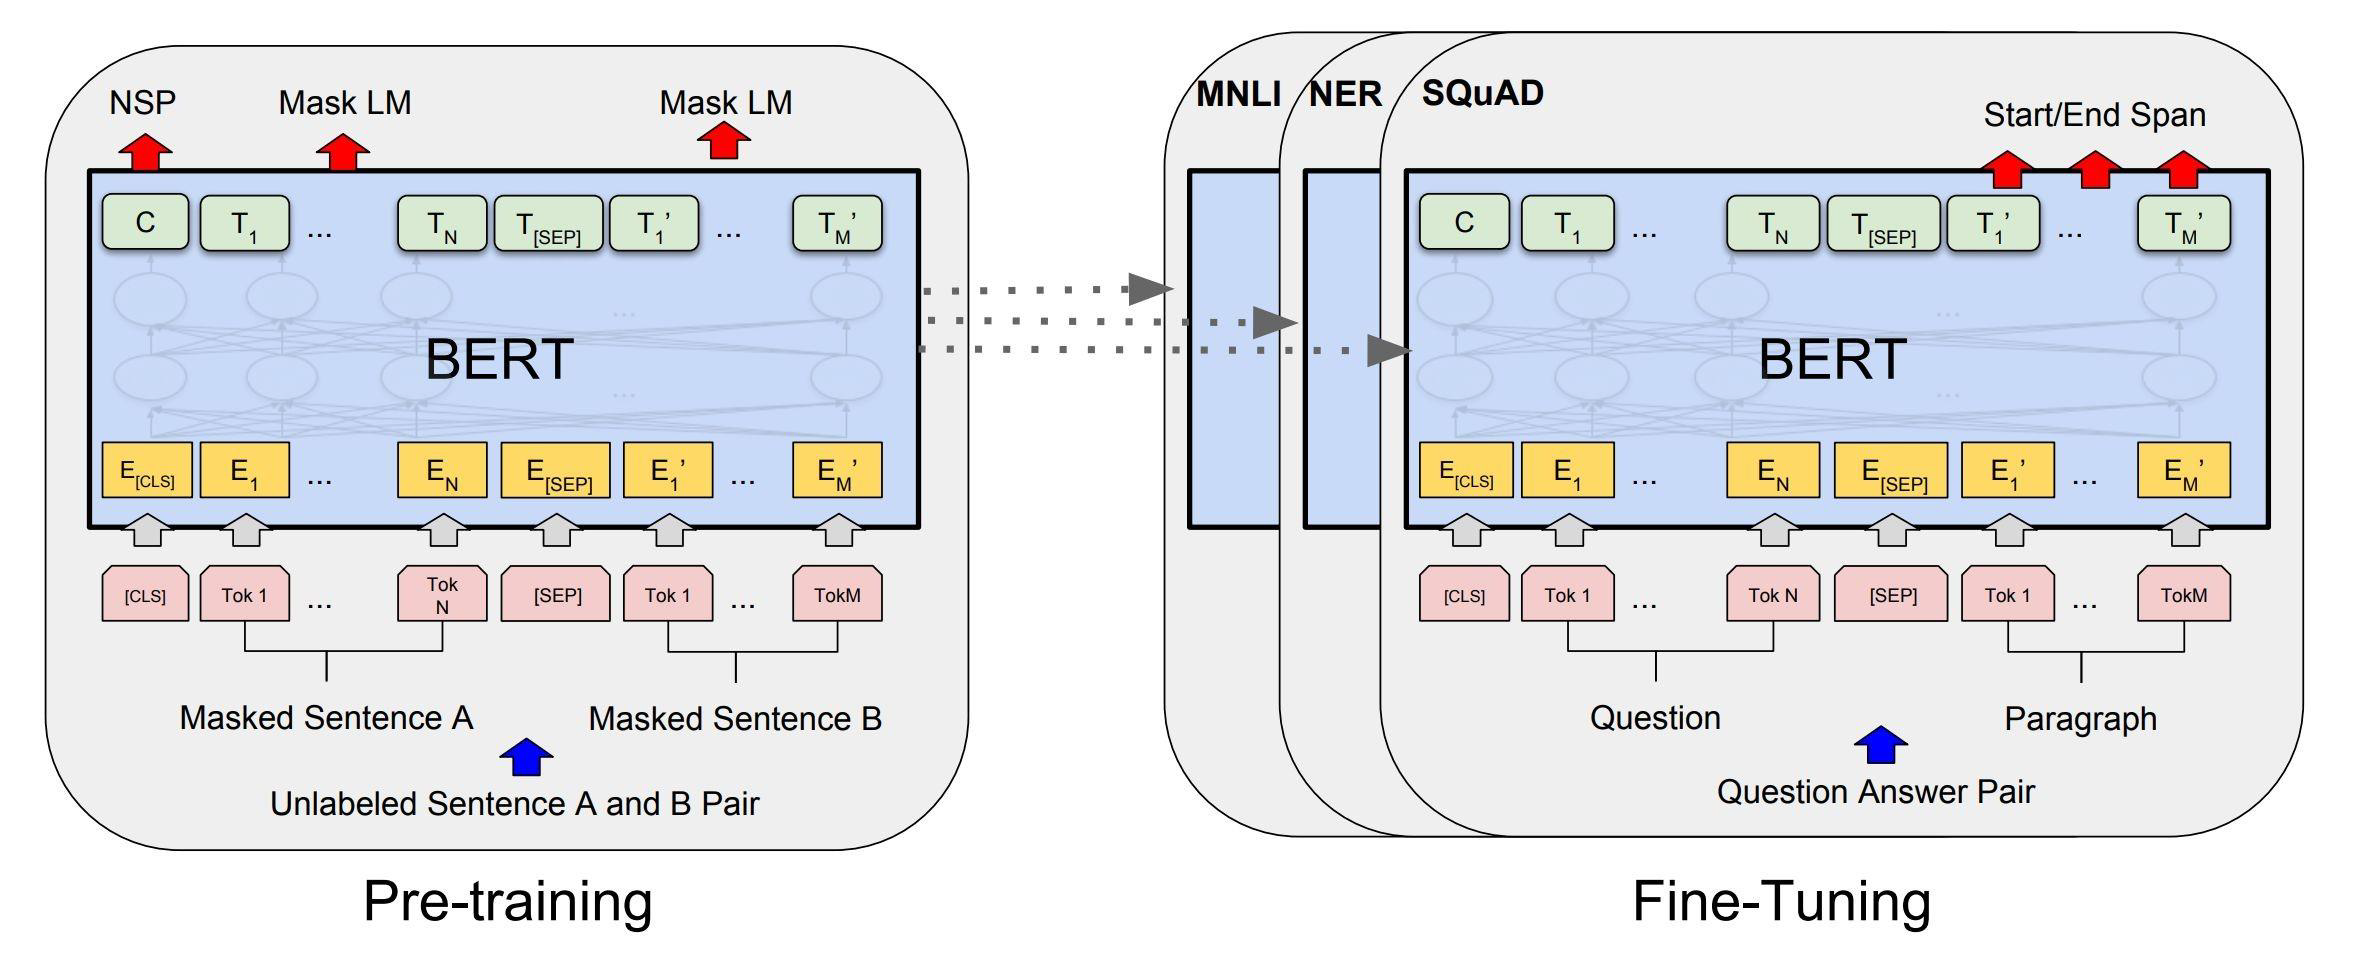
\includegraphics[width=0.7\linewidth]{images/seq-bert}
    \caption[BERT]{BERT}
    \label{fig:seq-bert}
\end{figure}

Observations:
\begin{myitem}
    \item Masked LM (compared to left-to-right LM) is very important on some tasks, Next Sentence Prediction is important on other tasks;
    \item Left-to-right model does very poorly on word level task (SQuAD), although this is mitigated by BiLSTM;
    \item Masked LM takes slightly longer to converge because we only predict $k$\% instead of 100\%, but absolute results are much better almost immediately;
    \item Big models help a lot.
\end{myitem}

\textbf{RoBERTa}, is a \textit{Robustly Optimized BERT Pretraining Approach}: trained BERT for more epochs and/or on more data, each combination is useful.

\textbf{ELECTRA}, \textit{Pre-training Text Encoders as Discriminators Rather Than Generators}, trains model to discriminate locally plausible text from real text.

These models are very accurate, but too large and expensive. Thus, to apply them to low-latency production services, companies apply \textbf{distillation}, or \textit{model compression}:
\begin{myitem}
    \item Train \textit{teacher}: use a big dataset and fine-tuning technique to train a model with maximum accuracy;
    \item Label a large amount of unlabeled input examples with Teacher;
    \item Train \textit{Student}: much smaller model which is trained to mimic Teacher output;
    \item Student's objective is typically Mean Square Error or Cross Entropy.
\end{myitem}
Distillation works much better than pre training + fine tuning with smaller model.
